\section{SAQI Application}
\label{sec:app}
We built a mobile and Web friendly SAQI application (Figure~\ref{fig:saqi_layout})\footnote{Web version of the app can be accessed live at \url{https://w3id.org/saqi/app}.} that makes use of the KG to answer questions related to air quality.\footnote{The uploaded data in KG consists of ~3.4 million triples mostly from sensors data collected over 4 months} To mitigate the knowledge barrier in understanding AQI, increase awareness related to air pollution and improve citizen engagement, the app is designed to address all the sections of the community, including the tech ill-literate people. This is achieved using features such as support for local language -- Hindi/English, heavy/large fonts, minimal user input, text-to-speech narration on every page and colourful graphics for AQI readings. The app consists of knowledge on air pollution and its effects which caters to specific social and spatial cohorts and also acts as AQI monitoring app that utilizes a KG built using SAQI ontology. 

\begin{figure}[ht]
\centering
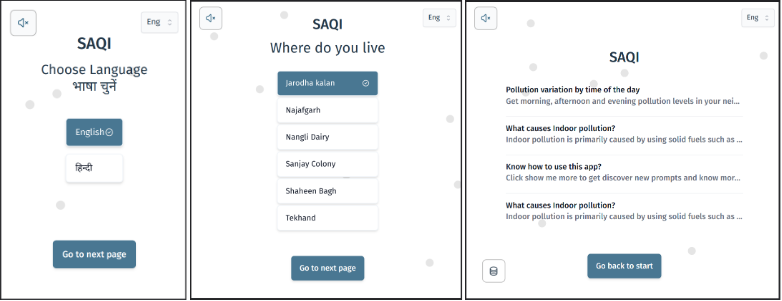
\includegraphics[ height=4.5cm]{figures/saqi_app_layout.png}
\caption{User interface of the SAQI app. Each screen has only one clickable input with large, clear fonts with minimal content} 
\label{fig:saqi_layout}
\end{figure}

A SPARQL endpoint (Figure~\ref{fig:saqi_sparql}) is also embedded in the application with eight queries on the pollution sensors data and the ethnography data from surveys. The SPARQL endpoint can be accessed from the app at  \url{https://w3id.org/saqi/app/#/sparql}. The ethnographic data, pollution data from local and central sensors are mapped to triples using RDF Mapping Language (RML) helper tool YARRML\footnote{\url{https://rml.io/yarrrml/}.}~\cite{YARRRML} that provides a high level format to define R2RML and RML rules. The generated triples are loaded into a server running Apache Jena Fuseki\footnote{\url{https://jena.apache.org/documentation/fuseki2/}.} as the triple store. A cron job running on the server updates the KG with the new triples and validates the KG using SHACL constraints.

 \begin{lstlisting}[label=lst:saqi-query,caption={An example of a SPARQL query used by saqi; output of this query is present in Table~\protect\ref{saqi-query-result}},float,frame=tb,captionpos=b,basicstyle=\ttfamily\small]
 
# The query returns average pollutants in specific time bands
  PREFIX rdf: <http://www.w3.org/1999/02/22-rdf-syntax-ns#>
  PREFIX rdfs: <http://www.w3.org/2000/01/rdf-schema#>
  PREFIX saqi: <https://kracr.iiitd.edu.in/ontology/saqi#>
  PREFIX xsd: <http://www.w3.org/2001/XMLSchema#>
  PREFIX sosa: <http://www.w3.org/ns/sosa/>
  
  SELECT (AVG(?pm10Instance) AS ?pm_10) 
  (AVG(?pm25Instance) AS ?pm_25) ?timesofday WHERE {
    ?obs_pm_25 a sosa:Observation .
    ?obs_pm_25 sosa:resultTime ?time .
    ?obs_pm_25 saqi:atPlace ?place .
    ?obs_pm_25 saqi:madeBySensor ?source .
    ?obs_pm_10 a sosa:Observation .
    ?obs_pm_10 sosa:resultTime ?time .
    ?obs_pm_10 saqi:atPlace ?place .
    ?obs_pm_10 saqi:madeBySensor ?source .
  	# Add location name or time interval filter
    FILTER (
      ?time > "2021-11-01T00:00:00+05:30"^^xsd:dateTime &&
      ?time < "2021-11-10T00:00:00+05:30"^^xsd:dateTime
    )
    ?obs_pm_25 sosa:observedProperty saqi:ParticulateMatter2_5Concentration .
    ?obs_pm_25 sosa:hasResult ?pm25Instance .
    ?obs_pm_10 sosa:observedProperty saqi:ParticulateMatter10Concentration .
    ?obs_pm_10 sosa:hasResult ?pm10Instance .
  	?place saqi:hasName ?placeName .
	  ?source rdfs:label ?dataSource .
    BIND (hours(?time) AS ?hour)
    OPTIONAL { FILTER (?hour <= 8)
      BIND("Morning" AS ?timesofday)
    }
    OPTIONAL { FILTER (?hour > 8 && ?hour <= 16)
      BIND("Afternoon" AS ?timesofday)
    }
    OPTIONAL { FILTER (?hour > 16 && ?hour <= 20)
      BIND("Evening" AS ?timesofday)
    }
    OPTIONAL { FILTER (?hour > 20)
      BIND("Night" AS ?timesofday)
    }
  } 
  GROUP BY ?timesofday
  LIMIT 10000
\end{lstlisting}

\begin{table}[!h]
\begin{center}
\caption{Result of SPARQL Query from Listing~\ref{lst:saqi-query}}
\label{saqi-query-result}
\begin{tabular}{|c c c|} 
 \hline
 pm\_10 & pm\_25 & timesofday \\ [0.5ex] 
 \hline\hline
 331.96637 & 282.92276 & Morning \\ 
 \hline
 381.802 & 332.8371 & Night \\
 \hline
 302.69052 & 260.283 & Afternoon \\
 \hline
 335.77588 & 285.6778 & Evening \\ [1ex] 
 \hline
\end{tabular}
\end{center}
\end{table}

 %\footnote{Apache Jena Fuseki \url{https://jena.apache.org/documentation/fuseki2/}.}
 
\begin{figure}[ht]
\centering
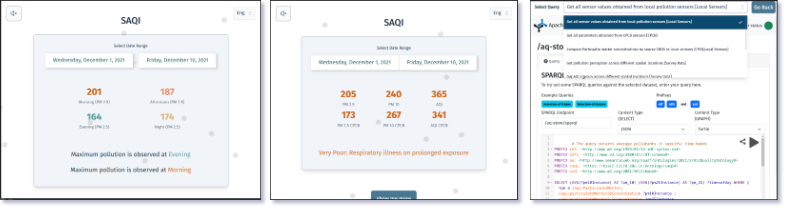
\includegraphics[ height=3.5cm]{figures/saqi_sparql.png}
\caption{Screenshots of the app using SPARQL queries to answer questions. The SPARQL endpoint screen is also shown here.} 
\label{fig:saqi_sparql}
\end{figure}

%\subsection{Methodology}

\subsection{Evaluation}
To evaluate the SAQI app, we conducted a user survey across the six locations where the local sensors were deployed. There were 60 participants spread across each of the six social cohorts. There were an equal number of male and female participants, and the age range of the participants was between 17 and 57 years. The questions to the participants were on media and digital literacy, AQI and air pollution awareness, the app's usability and utility, and community building after using the app. We used the Likert scale (1 to 5) for several questions, with 1 depicting the best case scenario and 5 the worst case. The feedback on the app was largely positive. The app got a usability score of $\sim$1.8, and a utility score of $\sim$2.1 on the understanding of AQI and $\sim$2.25 on suggestions to handle air quality in a local region. This is shown in Figure~\ref{fig:evaluation}. The survey also captures feedback on the improvements to the app, which is available after anonymization at \url{https://doi.org/10.5281/zenodo.10300235}. 

\begin{figure}
    \centering
    \begin{subfigure}[b]{0.38\textwidth}
        \centering
        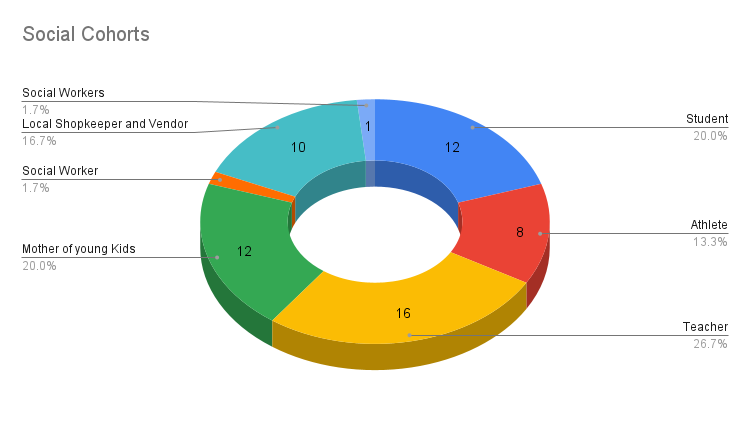
\includegraphics[width=\textwidth]{figures/evaluation2.png}
        \caption{Demographics}
        \label{fig:demographics_evaluation}
    \end{subfigure}
    \hfill
    \begin{subfigure}[b]{0.6\textwidth}
         \centering
         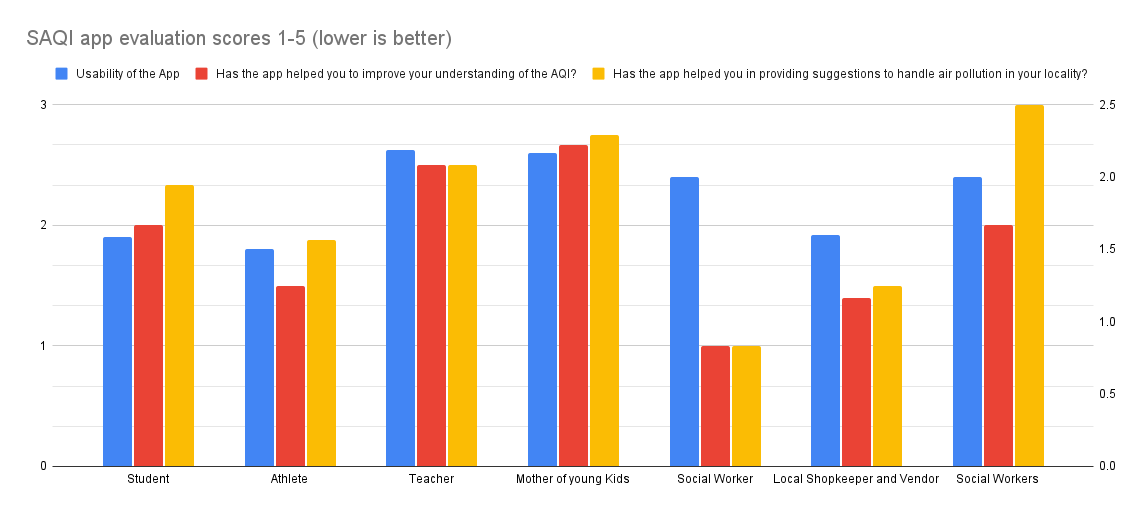
\includegraphics[width=\textwidth]{figures/evaluation.png}
         \caption{Evaluation scores}
         \label{fig:scores_evaluation}
     \end{subfigure}
    \caption{SAQI App evaluation results}
    \label{fig:evaluation}
\end{figure}

% \begin{figure}[ht]
% \centering

% 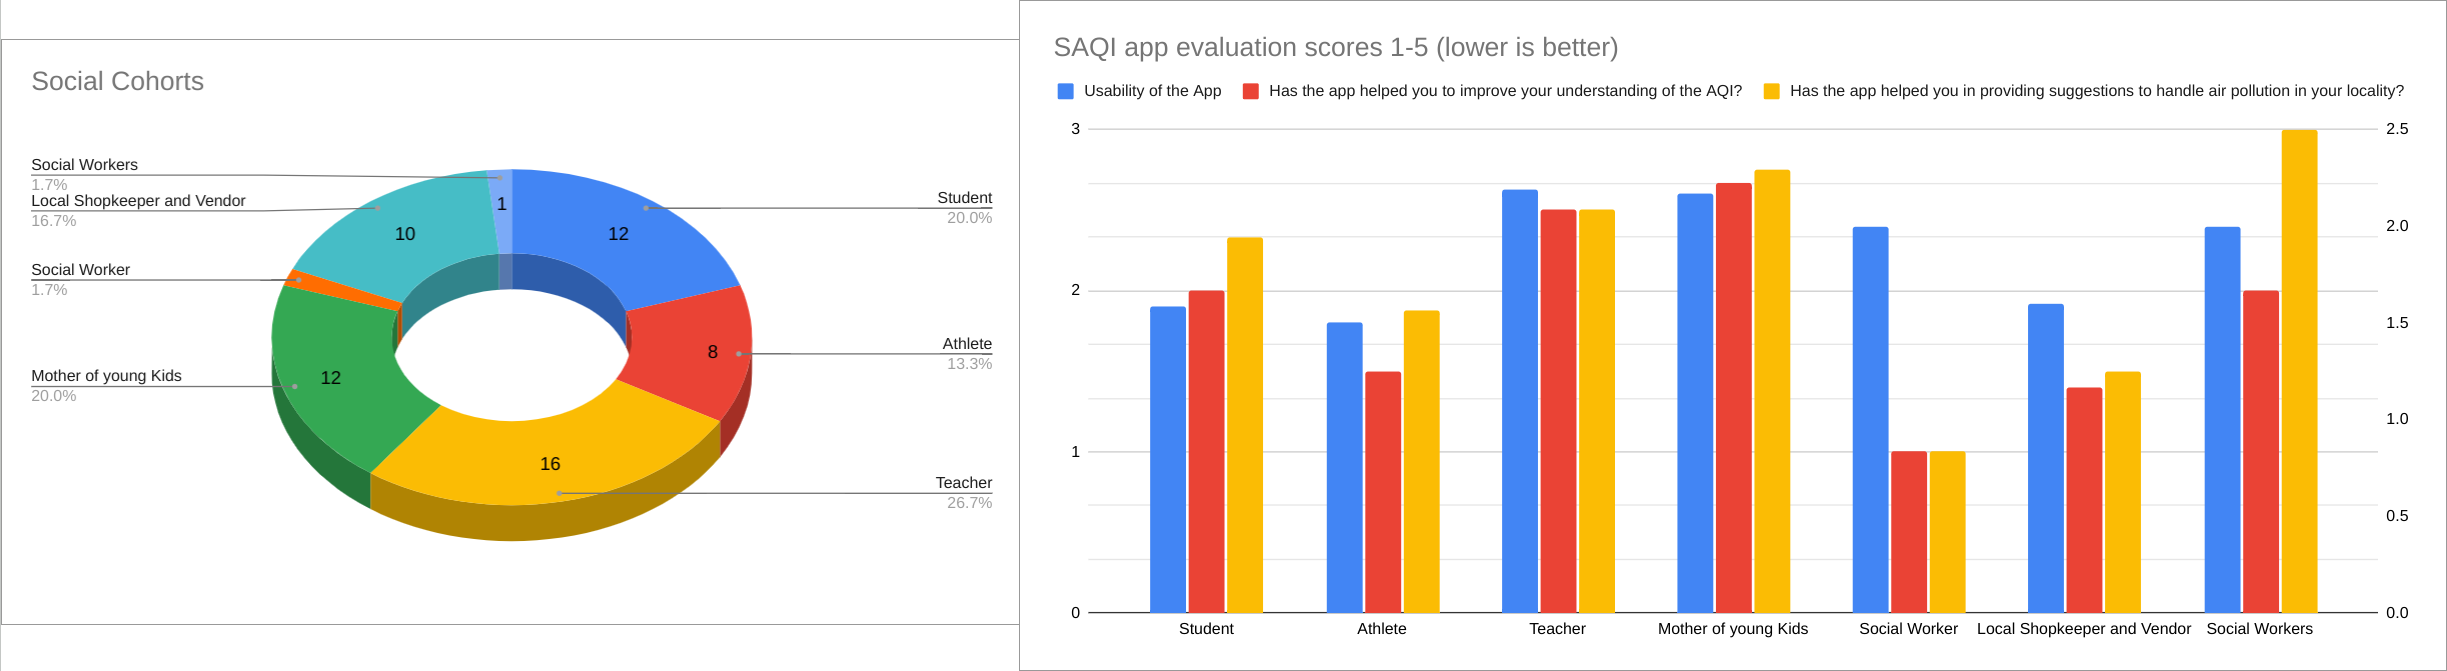
\includegraphics[height=3.5cm]{figures/saqiapp.png}
% \caption{Evaluation demographics and score for saqi app} 
% \label{fig:saqi_evaluation}

% \end{figure}

% TODO - add survey result summary, describe demographics - results - average rating questions(imp ones - usability, use fullness), summarize others. Add diagram - 3 graphs in one fig call them a,b,c.(like pie chart). Add some discussion points on them.
% Approx - 2 paras.

% DROP election